 \documentclass{article}

\title{Diploma}
\author{mishamilovidov}
\date{August 2025}

\usepackage{a4wide}
\usepackage[utf8]{inputenc}
\usepackage[T2A]{fontenc}
\usepackage[english,russian]{babel}
\usepackage{graphicx}
\usepackage{amsmath}
\usepackage{float}
\usepackage{hyperref}
\usepackage{amssymb}
\usepackage{bbm}
\usepackage{amsthm}
\usepackage{indentfirst}
\usepackage{float}
\usepackage{comment}
\usepackage[thinc]{esdiff}

\DeclareMathOperator{\sinc}{sinc}
%\DeclareMathOperator{\arctg}{arctg}
\DeclareMathOperator{\sgn}{sgn}
\DeclareMathOperator{\const}{const}
\DeclareMathOperator{\grad}{grad}
\renewcommand{\le}{\leqslant}
\renewcommand{\ge}{\geqslant}
\newcommand{\scalar}[2]{\left<#1,#2\right>}
\newcommand{\norm}[1]{\left\lVert #1 \right\rVert}
\newcommand{\abs}[1]{\left\lvert #1 \right\rvert}

\newtheorem{theorem}{Теорема}
\newtheorem{statement}{Утверждение}
\newtheorem{assumption}{Предположение}
\newtheorem*{remark}{Замечание}
\newtheorem{example}{Пример}
\theoremstyle{definition}
\newtheorem{definition}{Определение}[section]

\begin{document}
	\begin{titlepage}
		\begin{center}
			
\includegraphics[width=8cm, height=4cm]{msu.eps}
		\end{center}
		\begin{center}
			Московский государственный университет имени М.В. Ломоносова\\
			\vspace{0.1 cm}
			Факультет вычислительной математики и кибернетики\\
			\vspace{0.1 cm}
			Кафедра cистемного анализа
			
			\vspace{3cm}
			{\Large Миловидов Михаил Владимирович}\\
			\vspace{1cm}
			
			{\bf\LARGE Условия квазимонотонности для кусочно-аффинных систем дифференциальных уравнений} \\ \vspace{2cm}
			ВЫПУСКНАЯ КВАЛИФИКАЦИОННАЯ РАБОТА
			
		\end{center}
		\vspace{2cm}
		\begin{flushright}
			
			{\bf Научный руководитель:}\\
			к.ф.-м.н., доцент\\ 
			П.\,А. Точилин
			
		\end{flushright}
		
		\vfill
		
		\centerline{Москва, \the\year{}}
		
	\end{titlepage}

\tableofcontents

\newpage

\section{Введение}

Данная работа посвящена исследованию свойства квазимонотонности для систем дифференциальных уравнений. Квазимонотонные системы используются в различных прикладных областях и обладают полезными свойствами. Например, класс квазимонотонных систем является одним из самых важных классов динамических систем в математической биологии. Классический подход предполагает системы, не зависящие от функций управления. Описание таких систем можно найти в \cite{7}. В настоящее время также активно используется и исследуется класс систем, зависящих от управления (см. \cite{2}). Кроме математической биологии, данное свойство также используется в других прикладных областях, например, в исследовании транспортных потоков (см. \cite{8}).

Одним из главных свойств квазимонотонных систем является свойство сохранения порядка состояний системы. Это свойство напрямую связано с понятием частичного порядка, а также является альтернативным определением квазимонотонной системы. В классическом случае рассматривается случай положительного ортанта, но метод можно распространить как на остальные ортанты, так и на произвольный конус с некоторыми свойствами. Данные понятия хорошо описаны в \cite{2}.

В теории управления свойство квазимонотонности находит свое применение в создании внешних оценок на множества достижимости. Данный метод, наравне с другими, описан в \cite{1}. Преимущество метода заключается в том, что он вычислительно крайне прост, поэтому он может использоваться в задачах с большой размерностью пространства. Свойство также используется в более сложных задачах, таких как управление системой в условиях неопределенности на основании результатов измерений (см. \cite{4}).

Работа сосредоточена на исследовании распостраненного класса кусочно-аффинных функций. В ней рассмотренны различные частные случаи таких систем и раскрыты их свойства. В разделе 2 вводятся необходимые определения, а также некоторые свойства квазимонотонных функций. Далее определяются классы исследуемых систем, и проводится их исследование. В разделе 7 также доказана теорема о свойстве сохранения упорядоченности решений задачи Коши.

\section{Теоретические сведения}
Введем понятие квазимонотонной системы.
\begin{definition} 
    Система
    \begin{equation} \label{sys}
        \dot x = f(x),\, x \in \mathbb{R}^n,\, n \ge 2 
    \end{equation}
    называется квазимонотонной, если
    \[\forall i \in \overline{1,n},\ \forall \alpha_j \ge 0,\ j = \overline{1,n},\ j \ne i\]
    \begin{equation} \label{qm}
	    f_i(x_1+\alpha_1,\dots,x_{i-1} + \alpha_{i-1},x_i,x_{i+1}+\alpha_{i+1},\dots,x_n+\alpha_n) \ge f_i(x_1,\dots,x_n).
    \end{equation}
    Это свойство также называется монотонностью по внедиагональным элементам, или же условием Важевского.
\end{definition}
Это основное определение, которое будет использоваться в данной работе. В таком случае также говорят, что функция \(f(x)\) --- квазимонотонна.

Опишем далее некоторые свойства квазимонотонных функций. Для этого нам надо будет ввести определение квазимонотонной системы с функцией, зависящей от управления. Оно вводится аналогично стандартному случаю. Пусть задана система
\begin{equation} \label{usys}
	\begin{cases} 
		\dot x = f(t, x, u),\ t \in [t_0,t_1],\\
		x(t_0) = x_0 \in \mathcal{X}_0,\\
	\end{cases}
\end{equation}
где \(\mathcal{X}_0 \subset \mathbb{R}^n\) --- множество начальных значений, \(u = u(t) \in \mathcal{U}\ \forall t \in [t_0,t_1]\), \(\mathcal{U} \subset \mathbb{R}^m\) --- множество допустимых управлений. Решение системы с начальным значением \(x_0 \in \mathcal{X}_0\) в момент времени \(t_0\) и допустимым управлением \(u \in \mathcal{U}\) обозначается
\[
x(t; t_0, x_0, u),\ t \in [t_0,t_1].
\]
\begin{definition} 
	Система
	\begin{equation}
		\dot x = f(t, x, u),\, x \in \mathbb{R}^n,\, n \ge 2 
	\end{equation}
	называется квазимонотонной, если
	\[\forall i \in \overline{1,n},\ \forall \alpha_j \ge 0,\ j = \overline{1,n},\ j \ne i,\ \forall \beta_k \ge 0,\ k = \overline{1, m}\]

	\begin{multline}	\label{uqm}
		f_i(t, x_1+\alpha_1,\dots,x_{i-1} + \alpha_{i-1},x_i,x_{i+1}+\alpha_{i+1},\dots,x_n+\alpha_n, u_1 + \beta_1,\dots,u_m + \beta_m) \ge \\
		\ge f_i(t, x_1,\dots,x_n, u_1,\dots, u_m)\ \forall t \in [t_0,t_1].
	\end{multline}
\end{definition}


\begin{definition}
	Множество
	\[\mathcal{R}(t) = \mathcal{R}(t; t_0, \mathcal{X}_0, \mathcal{U}) = \{x \in \mathbb{R}^n: \exists x_0 \in \mathcal{X}_0,\ u \in \mathcal{U}: x = x(t; t_0, x_0, u)\},\ t \in [t_0,t_1]\]
	называется множеством достижимости системы в момент времени \(t\).
\end{definition}

\begin{definition} \label{hr}
	Множество
	\[
		[\underline{x}, \overline{x}] = \{x \in \mathbb{R}^n: \underline{x}_i \le x_i \le \overline{x}_i\ \forall i = \overline{1, n}\},\ \underline{x}, \overline{x} \in \mathbb{R}^n
	\]
	называется гиперотрезком или гиперпрямоугольником.
\end{definition}

Для квазимонотонных систем верно следующее утверждение:
\begin{statement}
    Пусть в системе (\ref{usys}) функция \(f\) непрерывно дифференцируема и для всех \(t \in [t_0,t_1],\ x \in \mathcal{X}_0,\ u \in \mathcal{U},\ i, j = \overline{1, n},\ i \neq j,\ k = \overline{1, m}\) выполнено
    \begin{equation} \label{jakobian}
    	\diffp{f_i}{{x_j}}(t, x, u) \ge 0,\ \diffp{f_i}{{u_k}}(t, x, u) \ge 0.
    \end{equation}
    Пусть также \(\mathcal{X}_0 \in [\underline{x}, \overline{x}],\ \mathcal{U} \subset [\underline{u},\overline{u}]\). Тогда
     \[
     	\mathcal{R}(t; t_0, \mathcal{X}_0, \mathcal{U}) \subset [x(t; t_0, \underline{x}, \underline{u}), x(t; t_0, \overline{x}, \overline{u})].
     \]
\end{statement}
Условие (\ref{jakobian}) в данном утверждении гарантирует квазимонотонности системы. Доказательство утверждения, а также более подробное описание можно найти в \cite{1}. Альтернативное определение квазимонотонности, а также связь со знаками производной при непрерывной дифференцируемости можно найти в \cite{2}.

Также введем понятие кусочно-аффинной функции.
\begin{definition}
	Функция \(f(x), x \in \mathbb{R}^n\) называется кусочно-аффинной, если она имеет вид
	\begin{equation} \label{pwadef}
		f(x) = \begin{cases}A^{(k)}x + b^{(k)},\quad x \in \Omega^{(k)},\end{cases}
	\end{equation}
	где
	\[\Omega \subset \mathbb{R}^n, \Omega = \bigsqcup_{k = 1}^m \Omega^{(k)},\, x \in \mathbb{R}^{n},\, A=[a_{ij}] \in \mathbb{R}^{n \times n},\, b \in \mathbb{R}^{n}.\]
	\[f_i^{(k)}(x) = \sum_{j=1}^{n} a_{ij}^{(k)}x_j + b_i^{(k)}.\]
\end{definition}

\section{Постановка задачи}
В данной работе мы будем исследовать условие квазимонотонности для частных видов кусочно-аффинных функций. В результате нужно получить некоторые необходимые и достаточные условия. Рассмотрим следующие виды функции \(f(x)\):
\begin{enumerate}
    \item \(\forall i = \overline{1,n}\ \, f_i(x) \) --- суперпозиция функций \(\min()\), \(\max()\) и арифметических операций.
    \item Функция \(f(x)\) определена на множестве \(\Omega \subset \mathbb{R}^n\), причем \(\Omega = \bigsqcup_{k = 1}^m \Omega^{(k)}\), где \(\Omega^{(k)}\) --- выпуклые многогранники, и функция \(f(x)\) на \(\Omega^{(k)}\) имеет вид \(f_i(x) = \sum_{j = 1}^{n} a_{ij}^{(k)}x_j + b_i^{(k)}\). Значения функции на границах обговариваются отдельно.
\end{enumerate}
Обе функции являются кусочно-аффинными.


\section{Общие свойства кусочно-аффинных систем}

\subsection{Аффинные системы}
Попробуем адаптировать свойства, описанные в разделе 2, для кусочно-аффинных систем. Для начала рассмотрим аффинную функцию вида
	\[f(x) = Ax + b,\, x \in \mathbb{R}^{n},\, A=[a_{ij}] \in \mathbb{R}^{n \times n},\, b \in \mathbb{R}^{n}.\]
\[f_i(x) = \sum_{j=1}^{n} a_{ij}x_j + b_i.\]
Запишем условие (\ref{qm}):
\[\forall i \in \overline{1,n}\ \ \forall \alpha_j \ge 0,\ j = \overline{1,n},\ j \ne i,\ \exists \tilde j:\ \alpha_{\tilde j} \ne 0 \\\]
\[\sum_{\substack{j=1 \\ j \neq i}}^{n} a_{ij}(x_j + \alpha_j) + a_{ii}x_i + b_i \ge \sum_{j=1}^{n} a_{ij}x_j + b_i.\]
Упростив, получаем
\[\sum_{\substack{j=1 \\ j \neq i}}^{n} a_{ij}\alpha_j \ge 0.\]
Учитывая, что условие должно быть выполнено для любых нетривиальных неотрицательных наборов \(\alpha\), для всех \(k = \overline{1, n},\, k \neq i\) рассмотрим наборы, где
\[\alpha_k = 1,\, \alpha_j = 0,\, j \neq k.\]
Таким образом, получаем необходимые условия квазимонотонности:
\begin{equation} \label{qmaff}
	a_{ij} \ge 0\ \forall i \neq j,\ i,j = \overline{1, n}.
\end{equation}
Нетрудно заметить, что эти условия являются также и достаточными условиями квазимонотонности. Таким образом, условия (\ref{qmaff}) являются критерием квазимонотонности аффинных систем.
\subsection{Кусочно-аффинные системы}
Теперь рассмотрим кусочно аффинные функции вида (\ref{pwadef}).
Аналогично случаю непрерывных аффинных систем, рассматривая отдельные области определения и выбирая \(\alpha\) так, чтобы не выводит точку из данной области, получаем необходимые условия квазимонотонности:
\begin{equation} \label{qmpwaff}
	a_{ij}^{(k)} \ge 0\ \forall i \neq j,\ i,j = \overline{1, n},\ k = \overline{1, m}.
\end{equation}
Но в общем случае кусочно-аффинных систем эти условия не являются достаточными. Мы также должны учитывать, как ведет себя функция на границах областей определения. При пересечении границы в любом направлении, задаваемом набором \(\alpha\), значение функции не должно убывать (то есть не должно быть скачка вниз). 


\section{Системы, являющиеся суперпозицией функций \(\min\) и \(\max\)}

\subsection{Случай неограниченной области}
Рассмотрим суперпозицию функций \(\min\) и \(\max\). Рассмотрим функции, у которых \(f_i\) являются суперпозициями функций \(\min\), \(\max\) а также арифметических операций \(+\) и \(-\) и операции умножения на константу.
\begin{example}
	\[\begin{cases}
		f_1(x) = 1 + \min(2x_1,x_2) + \min(x_1, 2x_2), \\
		f_2(x) = -\max(2x_1 - x_2, x_2, \min(3, x_1)).
	\end{cases}\]
	В данном примере функция \(f_2\) принимает следующий кусочно-аффинный вид:
	\[
		f_2(x) = \begin{cases}
			-2x_1 + x_2,\ x_1 \ge x_2,\\
			-x_2,\ x_1 < x_2. \\
		\end{cases}
	\]
	Заметим, что на одной из областей функция имеет отрицательный коэффициент перед переменной \(x_1,\ 1 \neq 2\). Поэтому, согласно критерию (\ref{qmpwaff}), функция \(f\) не является квазимонотонной.
\end{example}
Главное свойство, которое позволяет проверить квазимонотонность таких функций --- это их непрерывность. Так как каждый аргумент функций \(\min, \max\) является кусочно-аффинным, сами эти функции также будут являться кусочно-аффинными. В силу непрерывности нам не нужно волноваться о свойствах функции на границах, а достаточно лишь проверить необходимое условие монотонности в каждой области. Однако в общем случае для проверки нам придется найти явный вид кусочно-аффинной функции.
Рассмотрим случай простой суперпозиции:
\begin{equation} \label{fmax}
f_i(x) = \max(g_i^{(1)}(x),\dots,g_i^{(m_i)}(x))
\end{equation}
или
\begin{equation} \label{fmin}
f_i(x) = \min(g_i^{(1)}(x),\dots,g_i^{(m_i)}(x)),
\end{equation}
где
\[g_i^{(k)}(x) = \sum_{j=1}^n a_{ij}^{(k)} x_j + b_i^{(k)},\, i = \overline{1, n},\, k = \overline{1, m_i}.\]
Тогда получаем простое условие квазимонотонности функции, аналогичное (\ref{qmpwaff}):
\begin{equation} \label{qmmm}
	a_{ij}^{(k)} \ge 0\ \forall i \neq j,\ i,j = \overline{1, n},\ k = \overline{1, m_i}.
\end{equation}
Покажем, что, действительно, если в определении функции есть хотя бы один отрицательный коэффициент \(a_{ij}^{(k)}, i \neq j\), то условие квазимонотонности нарушается. Достаточно показать, что для одного из таких коэффициентов соответствующая функция \(g_i^{(k)}\) выбирается как максимум (минимум) для некоторого интервала \(x\). Рассмотрим сначала случай максимума и одного отрицательного коэффициента. Утверждение следует из того, что данная функция будет убывать по соответствующему аргументу, значит, для некоторого \(x\) вида \(x = (0,\dots,0,x_{j^*},0,\dots,0)\), где ненулевой элемент стоит на позиции, соответствующей отрицательному коэффициенту, ее значение превысит значение всех возрастающих функций при достаточно малом \(x_{j^*}\), а значит, будет значением кусочно-аффинной функции на некотором интервале. В случае нескольких отрицательных коэффициентов как минимум одна из них будет выбрана на некотором интервале. В случае минимума надо рассматривать достаточно большие \(x_{j^*}\).

К этому случаю можно свести некоторые более сложные виды функций, однако в общем случае не всегда можно утверждать об отсутсвии квазимонотонности при присутствии отрицательного внедиагонального коэффициента, так как соответствующая функция может не попасть в итоговую кусочно-аффинную функцию.

Рассмотрим несколько примеров, демонстрирующих применение данного критерия. Выберем \(n = 2\). Так как каждая из функций \(f_i,\ i = \overline{1, 2}\) исследуется независимо, сконцентрируем внимание на функции \(f_1\), выбрав \(f_2(x) \equiv 0\).
\begin{example}
	\[f_1(x) = \min(\frac{1}{2}(x_2 - x_1 - 1), x_2 - x_1, 2(x_2 - x_1 - 1)),\ f_2(x) \equiv 0.\]
	В данном случае все коэффициенты \(a_{12}^{(1)} = \frac{1}{2},\ a_{12}^{(2)} = 1,\ a_{12}^{(3)} = 2\) неотрицательны, поэтому функция является квазимонотонной. Отрицательные коэффициенты \(a_{11}^{(k)}\) нас не интересуют.
\end{example}
\begin{example} \label{exnotqm}
	\[f_1(x) = \max(x_2 + 1, -x_2),\ f_2(x) \equiv 0.\]
	В данном случае имеем отрицательный коэффициент \(a_{12}^{(2)} = -1\), поэтому функция не является квазимонотонной.
\end{example}

Рассмотрим также пример, в котором функция имеет более сложный вид, к которому не применим напрямую критерий (\ref{qmmm}).
\begin{example}
	\[f_1(x) = \max(0, \min(x_2, -x_2)),\ f_2(x) \equiv 0.\]
	Упростив, получаем, что \(f_1(x) \equiv 0\), поэтому функция является квазимонотонной. Однако здесь присутствует отрицательный коэффициент \(-1\) перед переменной \(x_2\).
\end{example}

\subsection{Случай ограниченной области}

В практических задачах часто возникает необходимость проверки квазимонотонности функций, являющихся суперпозицией функций \(\min\) и \(\max\) из предыдущего подпункта, на ограниченных областях. В частности, здесь будет рассматриваться случай области, имеющей вид гиперпрямоугольника или же гиперотрезка (см. определение \ref{hr}).

Продолжим рассматривать функции вида (\ref{fmax}) и (\ref{fmin}). Пусть областью, на которой изучается свойство квазимонотонности, является гиперотрезок \([\underline{x}, \overline{x}];\ \underline{x}, \overline{x} \in \mathbb{R}^n\). Главная особенность ограниченной области --- то, что некоторые функции \(g_i^{(k)}(x)\) могут не достигаться нигде на данной области (то есть ни в одной точке значение таких функций не является максимумом/минимумом среди всех остальных), а значит, даже наличие таких функций с отрицательными внедиагональными элементами в аргументах максимума/минимума может не нарушать условие квазимонотонности.

Далее будем рассматривать случай максимума, случай минимума рассматривается аналогично. Заметим, что если функция \(f_i\) является квазимонотонной, то она возрастает по всем внедиагональным переменным, и минимум достигается на множестве 
\[
	X_i = \{x = (\underline{x}_i, \dots, \underline{x}_{i-1}, x_i, \underline{x}_{i+1}, \dots, \underline{x}_n) \in \mathbb{R}^n,\ x_i \in [\underline{x}_i, \overline{x}_i]\},
\]
то есть на одном из ребер:
\[
	\min_{x \in [\underline{x}, \overline{x}]} f_i(x) = \min_{x \in X_i} f_i(x)
\]
На этом множестве функция является вогнутой, поэтому поиск минимума не составляет труда. Также из вогнутости функции по всем переменным можно сделать вывод, что если условие квазимонотонности нарушается, то минимум на множестве \(X_i\) (обозначим соответствующую точку \(x^*\)) больше не будет глобальным минимумом функции. А это значит, что, в таком случае, учитывая кусочно-аффинную структуру, функция будет убывать по одному из внедиагональных направлений, исходящих из этой точки, на некотором интервале, то есть существует направление \(j^* \neq i\) и функция \(g_i^{(k^*)}\) такая, что
\[
	g_i^{(k^*)}(x) = f_i(x),\ x \in [x^*,x^* + \varepsilon e_{j^*}],\ \varepsilon > 0,\ a_{ij^*}^{(k^*)} < 0,
\]
Это условие также можно проверить следующим образом: раз функция убывает на некотором интервале по внедиагональному направлению \(j^*\), то в точке минимума функции на \(X_i\) значение некоторой функции \(g_i^{(k^*)}\) с отрицательным коэффициентом \(a^{(k^*)}_{ij^*}\) должно быть строго больше, чем значения всех функций \(g_i^{(k)}\) с неотрицательным коэффициентом \(a^{(k)}_{ij^*}\). Таким образом, функция не будет являться квазимонотонной тогда и только тогда, когда для некоторого \(i\) в точке \(x^*\) максимум в \(f_i\) достигается на некой функции \(g_i^{(k^*)}\) отрицательным коэффициентом \(a^{(k^*)}_{ij^*}\), а значение всех функций \(g_i^{(k)}\) с неотрицательным коэффициентом \(a^{(k)}_{ij^*}\) строго меньше. Формально это записывается следующим образом:
\begin{equation} \label{bs}
	\exists\, j^* \neq i, \; \exists\, k^* \in \{1,\dots,m_i\} : \quad
	\begin{cases}
		g_i^{(k^*)}(x^*) = \max\limits_{k \in \{1,\dots,m_i\}} g_i^{(k)}(x^*), \\[6pt]
		a_{ij^*}^{(k^*)} < 0, \\[6pt]
		\forall\, k \in \{1,\dots,m_i\} : \; a_{ij^*}^{(k)} \ge 0 \ \Longrightarrow\ 
		g_i^{(k)}(x^*) < g_i^{(k^*)}(x^*).
	\end{cases}
\end{equation}

 Если же минимум на множестве \(X_i\) достигается более чем на одной точке, то нужно проверить все из них.

Рассмотрим пример, иллюстрирующий влияние области определения на квазимонотонность функции. Для этого рассмотрим функцию из примера \ref{exnotqm}:
\begin{example}
	\[n = 2,\ f_1(x) = \max(x_2 + 1, -x_2),\ f_2(x) \equiv 0.\]
	Рассмотрим несколько областей определения \(\mathcal{X}\):
	\begin{enumerate}
		\item 
		\[
			\mathcal{X} = [-\frac{1}{4},\frac{1}{4}] \times [-\frac{1}{4},\frac{1}{4}].
		\]
		Рассмотрим множество \(X_1 = [-\frac{1}{4},\frac{1}{4}] \times \{-\frac{1}{4}\} \), на котором должен достигаться минимум функции \(f_1\). Ясно, что она не зависит от \(f_1\), поэтому минимум достигается на всем множестве, и можно рассматривать любую точку, например, \(x^* = (0, -\frac{1}{4})\). В этой точке
		\[
			g_1^{(1)}(x^*) = -\frac{1}{4} + 1 = \frac{3}{4},\ g_1^{(2)}(x^*) = \frac{1}{4}.
		\]
		Так как максимум \(f_i\) достигается на функции с положительным коэффициентом \(a_{12}^{(1)} = 1\), функция является квазимонотонной на этой области (не выполнено второе условие в (\ref{bs})).
		
		\item 
		\[
			\mathcal{X} = [-\frac{1}{2},\frac{1}{2}] \times [-\frac{1}{2},\frac{1}{2}].
		\]
		Аналогично, \(X_1 = [-\frac{1}{2},\frac{1}{2}] \times \{-\frac{1}{2}\} \), \(x^* = (0, -\frac{1}{2})\),
		\[
			g_1^{(1)}(x^*) = -\frac{1}{2} + 1 = \frac{1}{2},\ g_1^{(2)}(x^*) = \frac{1}{2}.
		\]
		Получаем, что значения функций равны, и максимум достигается на обоих функциях. Однако одна из них имеет положительный коэффициент \(a_{12}^{(1)} = 1\). Таким образом, в (\ref{bs}) нарушается третье условие, а значит, функция также является квазимонотонной.
		
		\item 
		\[
			\mathcal{X} = [-1, 1] \times [-1, 1].
		\]
		Аналогично, \(X_1 = [-1,1] \times \{-1\} \), \(x^* = (0, -1)\),
		\[
			g_1^{(1)}(x^*) = -1 + 1 = 0,\ g_1^{(2)}(x^*) = 1.
		\]
		Здесь выполнены все условия в (\ref{bs}), а значит, функция не является квазимонотонной.
	\end{enumerate}
\end{example}

\section{Функция, заданная на симплексах}

\subsection{Введение функции, заданной на симплексах}
Рассмотрим некоторое разбиение области \(\Omega\) на симплексы, пересекающиеся только по граничным точкам. Идея состоит в том, что, задав функцию лишь на всех вершинах данных симплексов, мы сможем продолжить ее на всю область. Далее кратко опишем метод. Для более подробного описания см. \cite{9}, раздел 2, а также \cite{10}.

Обозначим все уникальные вершины симплексов за \(g_1,\dots,g_S\), где \(S\) --- число уникальных вершин. Для каждого симплекса \(\Omega^{(k)}\) обозначим координаты его вершин как \(g^{(k)}_1,\dots,g^{(k)}_{n+1}\). Тогда для любой точки \(x \in \Omega^{(k)}\) будет существовать единственный вектор барицентрических координат \(\alpha^{(k)} = \alpha^{(k)}(x) = (\alpha^{(k)}_1,\,\dots, \alpha^{(k)}_{n+1})\) такой, что
\[\sum_{i = 1}^{n + 1} \alpha^{(k)}_i = 1,\quad \alpha^{(k)}_i \ge 0\ \forall i = \overline{1, n+1},\quad \sum_{i = 1}^{n+1} \alpha^{(k)}_i g^{(k)}_i = x.\]
Дополним вектор \(x\) до  \(\tilde{x} = \begin{bmatrix} x \\ 1 \end{bmatrix}\), и пусть \(\tilde{G}^{(k)} = \begin{bmatrix} g^{(k)}_{1} & \dots & g^{(k)}_{n+1} \\ 1 & \dots & 1 \end{bmatrix} \in \mathbb{R}^{(n + 1) \times (n + 1)}\). Тогда \(\tilde{G}^{(k)} \alpha^{(k)}(x) = \tilde x\). Пусть \((\tilde{G}^{(k)})^{-1} = \begin{bmatrix} H^{(k)} & h^{(k)} \end{bmatrix}\). Получим, что \(\alpha^{(k)}(x) = H^{(k)} x + h^{(k)} \).

Пусть известны значения функции \(f\) на всех вершинах \(g_1,\dots,g_S\). При \(x \in \Omega^{(k)}\) справедливо следующее представление функции \(f\):
\[f(x) = F^{(k)}\alpha^{(k)}(x) = A^{(k)}x + b^{(k)},\]
где \[F^{(k)} = \begin{bmatrix} f(g^{(k)}_{1}) & \dots & f(g^{(k)}_{n+1}) \end{bmatrix} \in \mathbb{R}^{n\times(n+1)},\quad A^{(k)} = F^{(k)}H^{(k)} \in \mathbb{R}^{n\times n},\quad b^{(k)} = F^{(k)}h^{(k)} \in \mathbb{R}^{n}.\]
Таким образом, мы получили явный кусочно-аффинный вид функции на всей области определения и можем применить стандартный критерий квазимонотонности (\ref{qmpwaff}). 

В дальнейшем будем рассматривать функцию на одном симплексе, поэтому верхний индекс номера симплекса отбросим. Будем считать известными вершины симплекса: \(g_1,\dots, g_{n+1}\), и значения функции на них: \(f_i(g_1),\dots,f_i(g_{n+1}),\ i = \overline{1, n}\).

Рассмотрим простейший пример.
\begin{example}
	Пусть \(n = 2,\ S = 4,\ g_1 = (0, 0),\ g_2 = (0, 1),\ g_3 = (1, 0), g_4 = (1, 1)\), область определения \(\Omega\) --- квадрат с этими вершинами. Область разбивается на два симплекса:
	\(\Omega^{(1)}\) с вершинами \(g_1, g_2, g_3\) и \(\Omega^{(2)}\) с вершинами \(g_2, g_3, g_4\). Рассмотрим функцию \(f_1\) (Пусть \(f_2 \equiv 0\)). Пусть \(f_1(g_1) = 0,\ f_1(g_2) = 1, f_1(g_3) = -1,\ f_1(g_4) = 1\). Легко получить, что на симплексе \(\Omega^{(1)}\) функция будет иметь вид \(f_1^{(1)}(x) = x_2 - x_1\), а на \(\Omega^{(2)}\) --- \(f_1^{(2)}(x) = 2 x_2 - 1\). На каждой из областей внедиагональные элементы неотрицательны, а значит, функция является квазимонотонной на области определения.
\end{example}

\subsection{Общий случай}
Поиск обратной матрицы порой может быть затруднительным, поэтому попытаемся исследовать альтернативные способы проверки. В общем случае, к сожалению, задача проверки квазимонотонности функции не может быть сильно упрощена. Однако можно рассмотреть более стабильные методы. В частности, задачу нахождения матрицы и свободного вектора функции можно свести к решению линейных систем
\[
\begin{cases}
	\sum_{k = 1}^{n}g_{jk}a_{ik} + b_i = f_i(g_j),\ j = \overline{1, n+1}
\end{cases}
\]
относительно \(a_{ik}\) и \(b_i\) для всех \(i = \overline{1, n}\). В дальнейшем будем рассматривать одну систему для некоторого фиксированного \(i\). Можно заметить, что элементы \(a_{ii}\) и \(b_i\) не нужны для проверки, поэтому можно исключить их из системы для упрощения. Используем для этого уравнения при \(j = n+1\) и \(j = n\). Проделаем следующие шаги:

\begin{enumerate}
	
\item Сначала устраним \(b_i\) путем вычитания последнего уравнения из всех предыдущих. Получим систему из \(n\) уравнений:
\[
	\sum_{k = 1}^{n}(g_{jk} - g_{n+1,k})a_{ik} = f_i(g_j) - f_i(g_{n+1}),\ j = \overline{1, n}.
\]
\item Далее избавимся от слагаемого с диагональным элементом, для чего домножим каждое уравнение при \(j = \overline{1, n-1}\) на \(g_{n,i} - g_{n+1,i}\) и вычтем \(n\)-ое уравнение, умноженное на \(g_{j, i} - g_{n+1,i}\). Получим следующую систему:
\[
	\sum_{\substack{k = 1 \\ k \neq i}}^{n}\left((g_{n,i} - g_{n+1,i})(g_{jk} - g_{n+1,k}) - (g_{j, i} - g_{n+1,i})(g_{nk} - g_{n+1,k})\right)a_{ik} = 
\]
\[
	= (g_{n,i} - g_{n+1,i})(f_i(g_j) - f_i(g_{n+1})) - (g_{j, i} - g_{n+1,i})(f_i(g_n) - f_i(g_{n+1})),\ j = \overline{1, n-1}.
\]
\end{enumerate}
Таким образом, мы сократили размерность системы на 2. 

Обозначим 
\[\tilde g_{ijk} = (g_{n,i} - g_{n+1,i})(g_{jk} - g_{n+1,k}) - (g_{j, i} - g_{n+1,i})(g_{nk} - g_{n+1,k}),\]
\[\tilde f_{ij} = (g_{n,i} - g_{n+1,i})(f_i(g_j) - f_i(g_{n+1})) - (g_{j, i} - g_{n+1,i})(f_i(g_n) - f_i(g_{n+1})).\]
Тогда система принимает вид
\[
	\sum_{\substack{k = 1 \\ k \neq i}}^{n}\tilde g_{ijk}a_{ik} = \tilde f_{ij},\ j = \overline{1, n-1}.
\]
При этом благодаря аффинной независимости вершин симплекса система как была, так и остается невырожденной.

Фактически, мы свели задачу к проверке на неотрицательность всех коэффициентов новой линейной функции, полученной отбрасыванием диагонального коэффициента и свободного члена, по ее значениям в некоторых точках. Это эквивалентно проверке функции на монотонное неубывание по всем переменным. Для этого в общем случае, опять же, нужно решить соответствующую систему и посмотреть на знаки коэффициентов. 

Далее воспользуемся тем, что после шага 1 мы получаем систему, где коэффициенты матрицы \((g_{jk} - g_{n+1,k})\) не зависят от \(i\). Поэтому, решив систему методом Крамера (то есть приводя матрицу системы к единичной стандартными преобразованиями), в правой части системы мы получим формулу, в которую мы можем подставлять значения функций \(f_i\) на этих точках при \(i = \overline{1, n}\). Фактически, этот метод эквивалентен нахождению обратной матрицы, однако может быть более удобен.

Главное, что здесь можно заметить --- один раз решив задачу, мы получаем возможность проверки квазимонотонности функции на всех симплексах аналогичного вида, полученных из изначального сдвигом на некоторый вектор. Если в пространстве задана сетка из таких симплексов, то нам достаточно решить задачу лишь для всех уникальных из них, после чего мы получим простой способ проверки для всей сетки.

\subsection{Случай стандартного разбиения}
Стандартное разбиение задается следующим образом (см \cite{5}, раздел 6.3.2): рассматривается разбиение пространства \(n\)-мерными кубами, после чего каждый куб разбивается на симплексы способом, описанным ниже.

Для демонстрации разбиения рассмотрим единичный \(n\)-мерный куб
\[
	P = \{x \in \mathbb R^n: 0 \le x_i \le 1, i = \overline{1, n}\}.
\] 
Результаты для других кубов можно получить сдвигом и масштабированием единичного куба.

Каждый симплекс в разбиении данного \(n\)-мерного куба задается следующим образом: для некоторой перестановки \(\sigma = (\sigma_1, \dots, \sigma_n)\) чисел \(1,\dots,n\)
\[P_\sigma = \{x \in \mathbb R^n: 0 \le x_{\sigma_1} \le x_{\sigma_2} \le \dots \le x_{\sigma_n} \le 1\}.\]
Эти симплексы пересекаются лишь по границам и в объединении образуют весь \(n\)-мерный куб. Множество вершин таких симплексов имеет вид
\[
	\{g_1 = (0,\dots,0), g_2 = e_{\sigma_1}, g_3 = e_{\sigma_1} + e_{\sigma_2}, \dots, g_{n+1} = (1,\dots,1)\},
\]
где \(e_j,\ j = \overline{1, n}\) --- единичные векторы.

Рассмотрим примеры таких разбиений при \(n = 2\) и \(n = 3\).

\begin{figure}[H]
	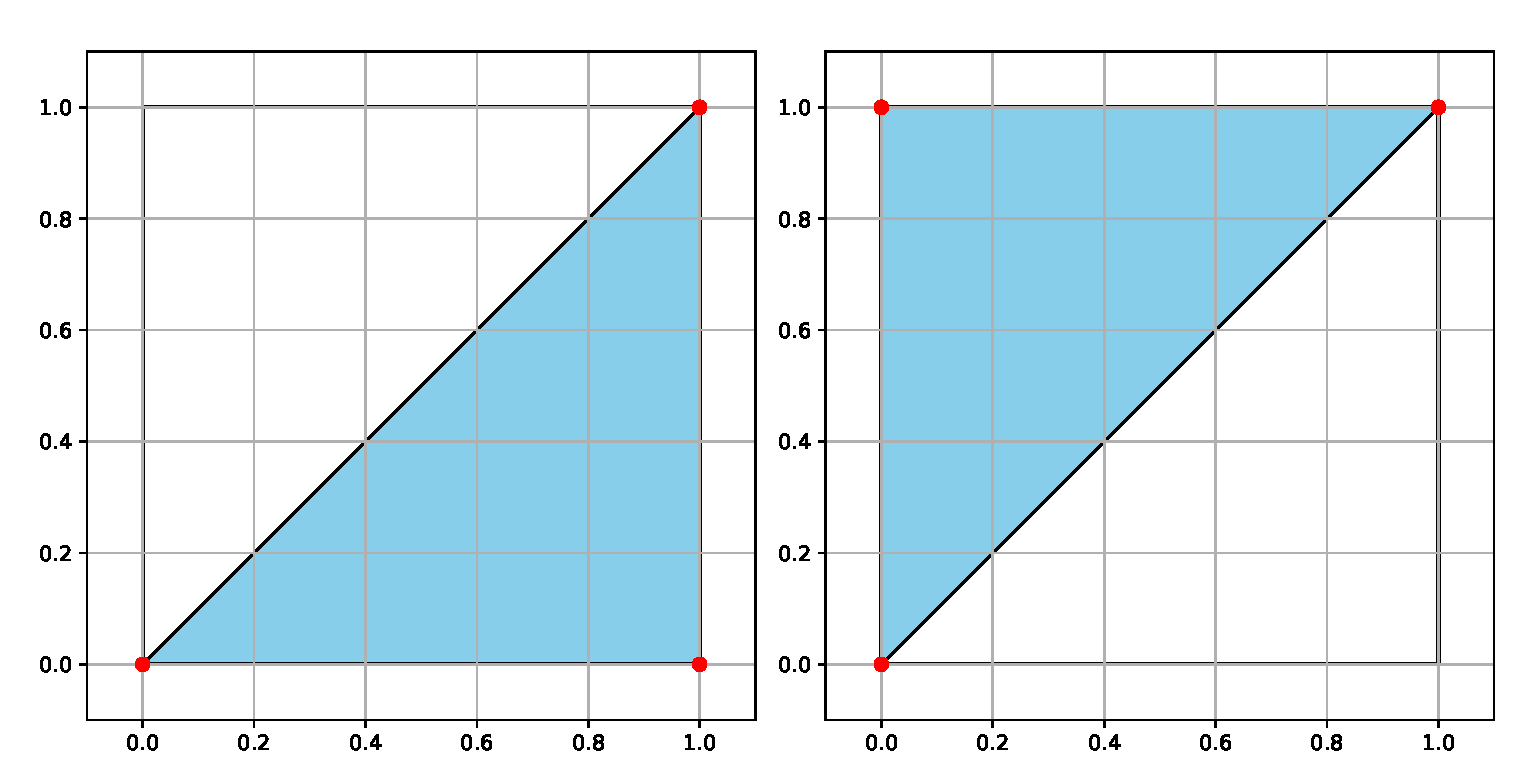
\includegraphics[width=1\textwidth]{graphics/ex1.eps}
	\caption{Стандартное разбиение в двумерном пространстве}
\end{figure}

\begin{figure}[H]
	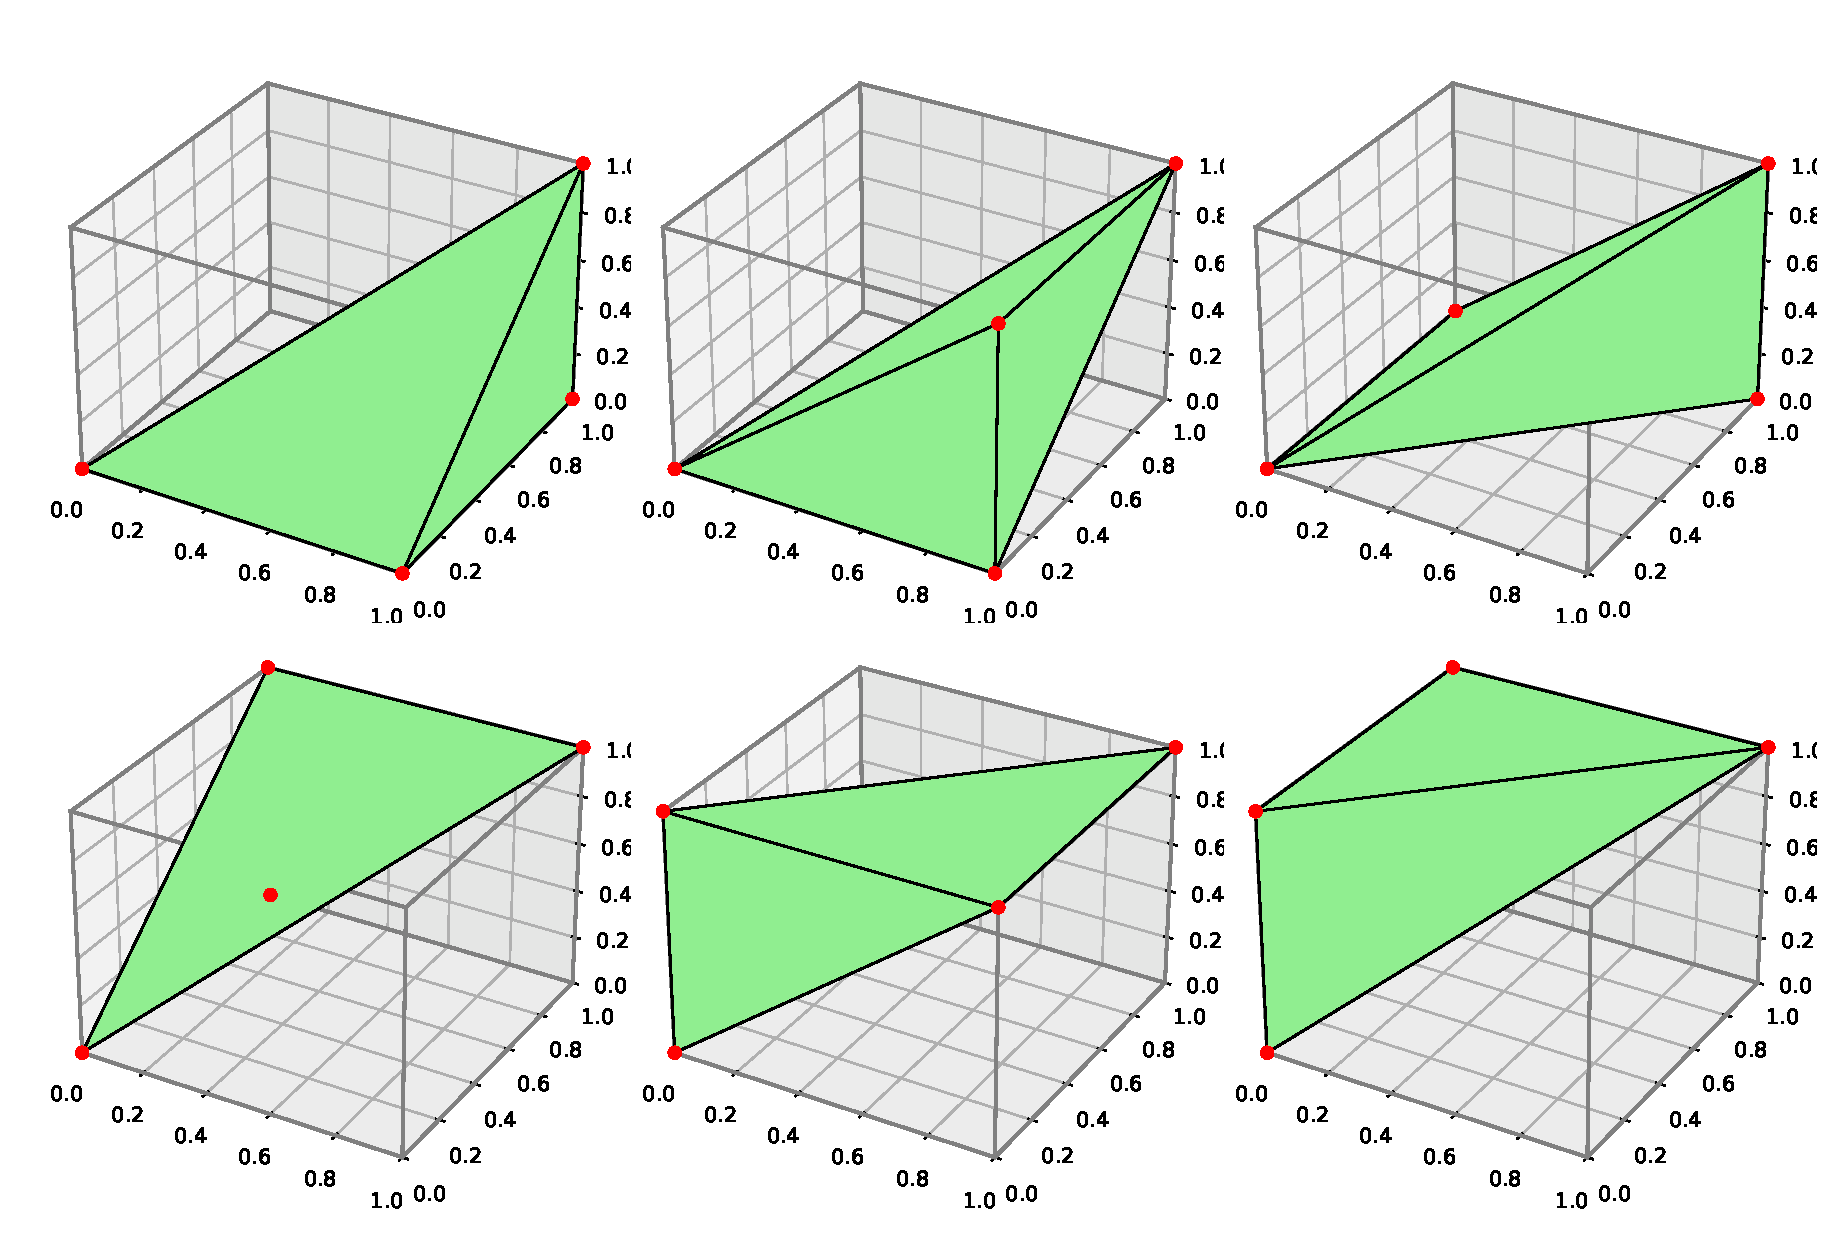
\includegraphics[width=1\textwidth]{graphics/ex2.eps}
	\caption{Стандартное разбиение в трехмерном пространстве}
\end{figure}

Преимущество таких симплексов состоит в том, что они легко поддаются исследованию на квазимонотонность. Действительно, если принять, что \(\sum_{k = 1}^{0} a_{ik} = 0\), получим:
\[f(g_{j+1}) - f(g_j) = \sum_{k = 1}^{j} a_{ik} - \sum_{k = 1}^{j-1} a_{ik} = a_{ij}.\]
Таким образом, условием квазимонотонности становится
\[f(g_{j+1}) - f(g_j) \ge 0\ \forall i = \overline{1, n},\ j = \overline{1, n},\ j\neq i.\]
Это эквивалентно тому, что при проходе вершин подряд функциия \(f_i\) возрастает, за исключением перехода от \(i\) к \(i+1\) вершине.

При проверке этих условий для всех симплексов \(n\)-мерного куба многие условия будут повторяться, поэтому можно проверять их сразу для всего куба. Они принимают следующий вид: для всех соседних вершин
\[\alpha = (\alpha_1, \dots, \alpha_{j-1}, 0, \alpha_{j+1},\dots, \alpha_n),\ \beta = (\alpha_1, \dots, \alpha_{j-1}, 1, \alpha_{j+1},\dots, \alpha_n),\]
\[i = \overline{1, n},\ j = \overline{1, n},\ j\neq i,\ \alpha_j \in \{0, 1\}\]
должно быть выполнено
\[f_i(\beta) - f_i(\alpha) \ge 0.\]

Рассматривая все пространство, мы также будем иметь повторяющиеся условия, поэтому стоит рассмотреть эти условия в общем виде. Они принимают следующий вид: для всех соседних вершин
\[\alpha = (\alpha_1, \dots, \alpha_{j-1}, \alpha_j, \alpha_{j+1},\dots, \alpha_n),\ \beta = (\alpha_1, \dots, \alpha_{j-1}, \alpha_j + 1, \alpha_{j+1},\dots, \alpha_n),\]
\[i = \overline{1, n},\ j = \overline{1, n},\ j\neq i,\ \alpha_j \in \mathbb Z\]
таких, что \(\alpha, \beta\) находятся в области определения функции, должно быть выполнено
\[f_i(\beta) - f_i(\alpha) \ge 0.\]
Все условия, полученные в данном подпункте, являются необходимыми и достаточными условиям квазимонотонности.

Рассмотрим простой пример исследования на монотонность функции, заданной на стандартном разбиении.
\begin{example}
	Пусть \(n = 2,\ g_1 = (0, 0),\ g_2 = (0, 1),\ g_3 = (1, 0), g_4 = (1, 1)\), область определения \(\Omega\) --- квадрат с этими вершинами. Область разбивается на два симплекса: \(\Omega^{(1)}\) с вершинами \(g_1, g_2, g_4\) и \(\Omega^{(2)}\) с вершинами \(g_1, g_3, g_4\). Пусть \(f_1(g_1) = 1,\ f_1(g_2) = 2, f_1(g_3) = 3,\ f_1(g_4) = 4;\ f_2(g_1) = 1,\ f_2(g_2) = -1, f_2(g_3) = 2,\ f_2(g_4) = 0 \). Исходя из полученных результатов, функция \(f\) будет монотонной тогда и только тогда, когда выполнены следующие неравенства:
	\[
		f_1(g_2) \ge f_1(g_1),\ f_1(g_4) \ge f_1(g_3);\ f_2(g_3) \ge f_2(g_1),\ f_2(g_4) \ge f_2(g_2).
	\]
	Так как в данном случае все они выполняются, функция \(f\) является квазимонотонной.
\end{example}

\section{Обобщенная квазимонотонность}

В разделе 2 были кратко упомянуты свойства квазимонотонных функций. В этом разделе приводится теорема, которая вводит более обобщенное понятие квазимонотонности (которая позволяет иметь как неубывание, так и невозрастание по различным внедиагональным переменным) и показывает основное свойство таких функций применительно к задачам Коши (сохранение упорядоченности решений), а также ее доказательство.
\begin{theorem}
	\begin{equation}
		\dot x = f(t, x),\ t\in [t_0,t_1],\ x \in \Omega \subset \mathbb{R}^n,
	\end{equation}
	Функция \(f(t, x)\) непрерывна по \(t\), удовлетворяет условию Липшица по \(x \in \Omega\). Зафиксируем два вектора \(y', y'' \in \Omega\), для которых
	\[\sigma_i y_i' \le \sigma_i y_i''\ \forall i = \overline{1, n},\ \exists j: \sigma_jy_j' < \sigma_j y_j'',\]	
	для некоторых фиксированных чисел \(\sigma_i \in \{-1, 1\},\ i = \overline{1, n}\). Пусть функция \(f(t, x)\) удовлетворяет условию квазимонотонности по внедиагональным элементам следующего вида:
	\begin{multline}
		\sigma_i f_i(t, x_1 + \sigma_1 \alpha_1,\dots, x_{i - 1} + \sigma_{i-1} \alpha_{i-1}, x_i, x_{i+1} + \sigma_{i+1} \alpha_{i+1}, \dots, x_n + \sigma_n \alpha_n) \ge \sigma_i f_i(t, x_1,\dots,x_n)
		\\ \forall t \in [t_0, t_1], x = (x_1,\dots,x_n) \in \Omega,\ \alpha = (\alpha_1,\dots,\alpha_n) \in \mathbb{R}^n_+,\ i = \overline{1, n}.
	\end{multline}
	Пусть \(x'(t),\ t \in [t_0, t_1]\) --- решение задачи Коши
	\begin{equation}
	\begin{cases} \label{zk1}
		\dot x' = f(t, x'), \\
		x'(t_0) = y'. \\
	\end{cases}
	\end{equation}
	Аналогично определено решение \(x''(t),\ t \in [t_0, t_1]\) задачи Коши
	\begin{equation}
	\begin{cases} \label{zk2}
		\dot x'' = f(t, x''), \\
		x''(t_0) = y''. \\
	\end{cases}
	\end{equation}
	Тогда \(\forall t \in [t_0,t_1]\) справедливы следующие неравенства:
	\begin{equation}
		\sigma_i x_i'(t) \le \sigma_i x_i''(t)\ \forall i = \overline{1,n}.
	\end{equation}
\end{theorem}

Сначала докажем данную теорему для модифицированной задачи.
Введем новую функцию
\[
g(t, x'''): g_i(t, x''') = f_i(t, x''') + \sigma_i \varepsilon \ \forall i = \overline{1, n},\ \varepsilon > 0.
\]
Рассмотрим модифицированную задачу Коши:
\begin{equation}
\begin{cases} \label{zk3}
	\dot x''' = g(t, x'''), \\
	x'''(t_0) = y''. \\
\end{cases}
\end{equation}
Предположим противное:
\begin{equation} \label{aa}
\exists i \in \{1,\dots,n\},\ \tau_1 \in [t_0, t_1]:\ \sigma_ix_i'(\tau_1) > \sigma_i x_i'''(\tau_1), \text{ или же } \sigma_i x_i'''(\tau_1) - \sigma_i x_i'(\tau_1) < 0.
\end{equation}
В силу непрерывности решения это означает, что
\[
	\exists \tau < \tau_1: x_i'(\tau) = x_i'''(\tau)
\]
Рассмотрим первый такой момент \(\tau\) (момент нарушения упорядоченности решений), для которого выполнено:
\[
	x_i'(\tau) = x_i'''(\tau);\ \sigma_j x_j'(\tau) \le \sigma_j x_j'''(\tau)\  \forall j \ne i,\ j = \overline{1,n};
\]
\[
	\sigma_i x_i'(t) > \sigma_i x_i'''(t)\ \forall t \in (\tau,\tau+\varepsilon_1),\ +\varepsilon_1 > 0.
\]
В силу условий выше,
\[
	g_i(\tau, x'''(\tau)) - f(\tau, x'(\tau)) \ge 0.
\]
Однако, учитывая условие квазимонотонности,
\[
	\sigma_i f_i(\tau, x'(\tau)) \le \sigma_i f_i(\tau,x'''(\tau)),
\]
мы получаем неравенство
\[
	\sigma_i f_i(\tau, x'(\tau)) < \sigma_i g_i(\tau,x'''(\tau)),
\]
что дает нам противоречие, а значит, предположение (\ref{aa}) неверно.

Для доказательства самой теоремы перейдем к пределу при \(\varepsilon \to 0\). Для задач Коши (\ref{zk2}) и (\ref{zk3}) выполнены все условия теоремы о непрерывной зависимости задачи Коши от параметра (см. \cite{6}, 1.1.1), а значит,
\[
	\max_{t \in [t_0, t_1]} \abs{x''(t) - x'''(t)} \le С\varepsilon,
\]
где \(С\) --- некоторая константа. Таким образом, справедливо неравенство
\[
	\sigma_i x_i'(t) \le \sigma_i x_i''(t) + \sigma_i C\varepsilon \ \forall i = \overline{1,n},\ t\in [t_0, t_1],\ \varepsilon > 0.
\]
Переходя к пределу при \(\varepsilon \to 0\), получаем
\[
\sigma_i x_i'(t) \le \sigma_i x_i''(t)\ \forall i = \overline{1,n},\ t\in [t_0, t_1],
\]
что и требовалось доказать.

Отметим, что от данного условия квазимонотонности к стандартному можно перейти, произведя замену переменных. Однако иногда удобнее этого не делать, чтобы не терялся практический смысл переменных.

Для обобщенной квазимонотонности можно проводить рассуждения, аналогичные описанным в предыдущих разделах. Например, критерий (\ref{qmaff}) в таком случае превращается в следующее:
\begin{equation}
	\sigma_i \sigma_j a_{ij} \ge 0\ \forall i \neq j,\ i,j = \overline{1, n}.
\end{equation}
Критерии (\ref{qmpwaff}) и (\ref{qmmm}) изменяются аналогичным образом.
\begin{comment}
\subsection{Случай положительного ортанта}

Зададимся вопросом поиска условий на вершины симплекса, при которых можно проверить квазимонотонность без решения системы. Идея состоит в том, чтобы в приведенной системе все коэффициенты \(\tilde g_{ijk}\) были неотрицательны. При таком условии, исходя из невырожденности системы (а значит и линейной независимости строк матрицы системы, которые являются точками, в которых известно значение редуцированной функции), достаточно проверить неотрицательность всех значений \(\tilde f_{ij}\), ведь у линейной функции значение в нуле --- ноль.

Возникает вопрос: какие условия достаточно наложить на вершины \(g_{jk}\), чтобы можно было перейти к такой приведенной системе? Покажем, что достаточно рассматривать симплексы, у которых некоторая вершина (пусть это будет \(g_{n+1}\)) покоординатно меньше или равна всем остальным вершинам. Частным случаем такого симплекса является симплекс, у которого одна вершина расположена в нуле, а остальные --- в положительном ортанте (включая границы). Остальные же симплексы получаются при помощи сдвига нулевой вершины таких симплексов. При таком условии на первом шаге упрощения системы из предыдущего пункта мы гарантируем неотрицательность всех коэффициентов промежуточной системы. Далее модифицируем второй шаг: вместо вычитания 
\end{comment}

\begin{thebibliography}{99}
	\bibitem{1} Meyer, P.-J. Interval Reachability Analysis / P.-J. Meyer, A. Devonport, M. Arcak. --- Springer, 2021. --- 115 p.
	\bibitem{2} Angeli, D. Monotone control systems / D. Angeli, E.D. Sontag // IEEE Trans. Automat. Control. --- 2003. --- V. 48, № 10. — P. 1684–1698.
	\bibitem{3} Ramdani N. Computing reachable sets of uncertain nonlinear monotone systems / N. Ramdani, N. Meslem, Y. Candau // Nonlin. Anal. Hybrid Syst. --- 2010. --- V. 4, № 2. --- P. 263–278.
	\bibitem{4} Точилин П.А. О задаче целевого управления монотонной системой на основании результатов измерений. / Точилин П.А. // Дифференц. уравнения. --- 2025. --- Т. 61, № 11. --- С. 1527–1545.
	\bibitem{5} De Loera J. A. Triangulations: structures for algorithms and applications. / De Loera J. A., Rambau J., Santos F. --- Springer, 2010. --- 535 p.
	\bibitem{6} Денисов А.М. Обыкновенные дифференциальные уравнения. Часть 2. / Денисов А.М., Разгулин А.В. --- МАКС Пресс Москва, МГУ, 2009 г. --- 232 c.
	\bibitem{7} Smith H.L. Monotone dynamical systems: An introduction to the theory of competitive and cooperative systems. / Smith H.L. // Mathematical Surveys and Monographs. --- AMS, Providence, RI, 1995. --- V. 41. --- 174 p.
	\bibitem{8} Куржанский, А.Б. Роль макромоделирования в активном управлении транспортной сетью / А.Б. Куржанский, А.А. Куржанский, П. Варайя // Тр. МФТИ. --- 2010. --- Т. 2, № 4. --- С. 100–118.
	\bibitem{9} Точилин П.А. О построении кусочно-аффинной функции цены в задаче оптимального управления на бесконечном отрезке времени. / Точилин П.А. // Тр. Ин-та математики и механики УрО РАН. --- 2020. --- Т. 26, № 1. --- C. 223-238.
	\bibitem{10} Пшеничный Б.Н. Выпуклый анализ и экстремальные задачи. / Пшеничный Б.Н. --- М.: Наука, 1980. --- 319 с.
\end{thebibliography}

\end{document}

